\documentclass[12pt]{article}
\usepackage[left=2cm,right=2cm,top=2cm,bottom=2cm,bindingoffset=0cm]{geometry}
\usepackage{fontspec}
\usepackage{polyglossia}
\usepackage{amssymb}
\setdefaultlanguage{russian}
\setmainfont[Mapping=tex-text]{CMU Serif}

\begin{document}
%% Весь этот текст можно удалить
%% ====== от сих =====
\begin{center}
  \LARGE Формальные языки 

  \Large домашнее задание до 23:59 27.04
\end{center}
\bigskip

\begin{enumerate}
  \item Реализовать алгоритм синтаксического анализа графов: на входе ориентированный граф $G=(V,E)$ и граматика $C(S)=(\Sigma, N, P, S)$ в нормальной форме Хомского, на выходе --- множество троек $(v_1,v_2,n)$, где $v_1, v_2 \in V, n \in N$, таких, что существует путь $p$ из $v_1$ в $v_2$, такой, что $\Omega(p) \in L(C(n))$.
  \item Применить реализованный алгоритм для поиска tRNA в метагеномной сборке. Сборка --- ориентиорванный гаф с метками из $\Sigma^*$, где $\Sigma=\{a,c,g,t\}$. Суммарная длина всех меток не менее 1000. Грамматику для tRNA необходимо составить по следующему описанию (см картинку). Длина каждой петли от 2 до 4 символов, высота каждого столбика не меньше 2 пар.
  \begin{center} 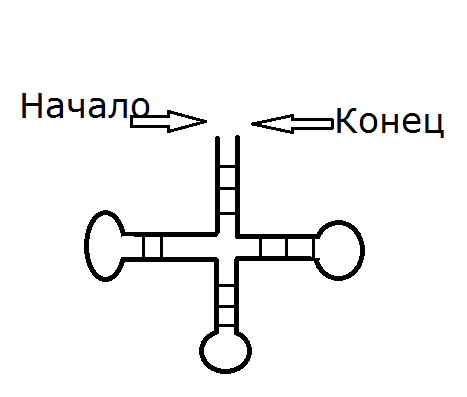
\includegraphics[width=0.65\linewidth]{тРНК.png} \end{center}
  Результат:
  \begin{itemize}
  \item Грамматика tRNA
  \item Генератор метагеномных сборок
  \item Приложение, осуществляющее поиск tRNA в метагеномных сборках
  \end{itemize}
  %\begin{verbatime}
  %stem<S> : a stem<S> c | c stem<S> a | g stem<S> t | t stem<S> g | S
  %\end{verbatime}
\end{enumerate}  


%% ===== и до сих =====
\end{document}
